\chapter{User requirements definition}

\section{Use Cases Diagramm}
\begin{figure}[H]
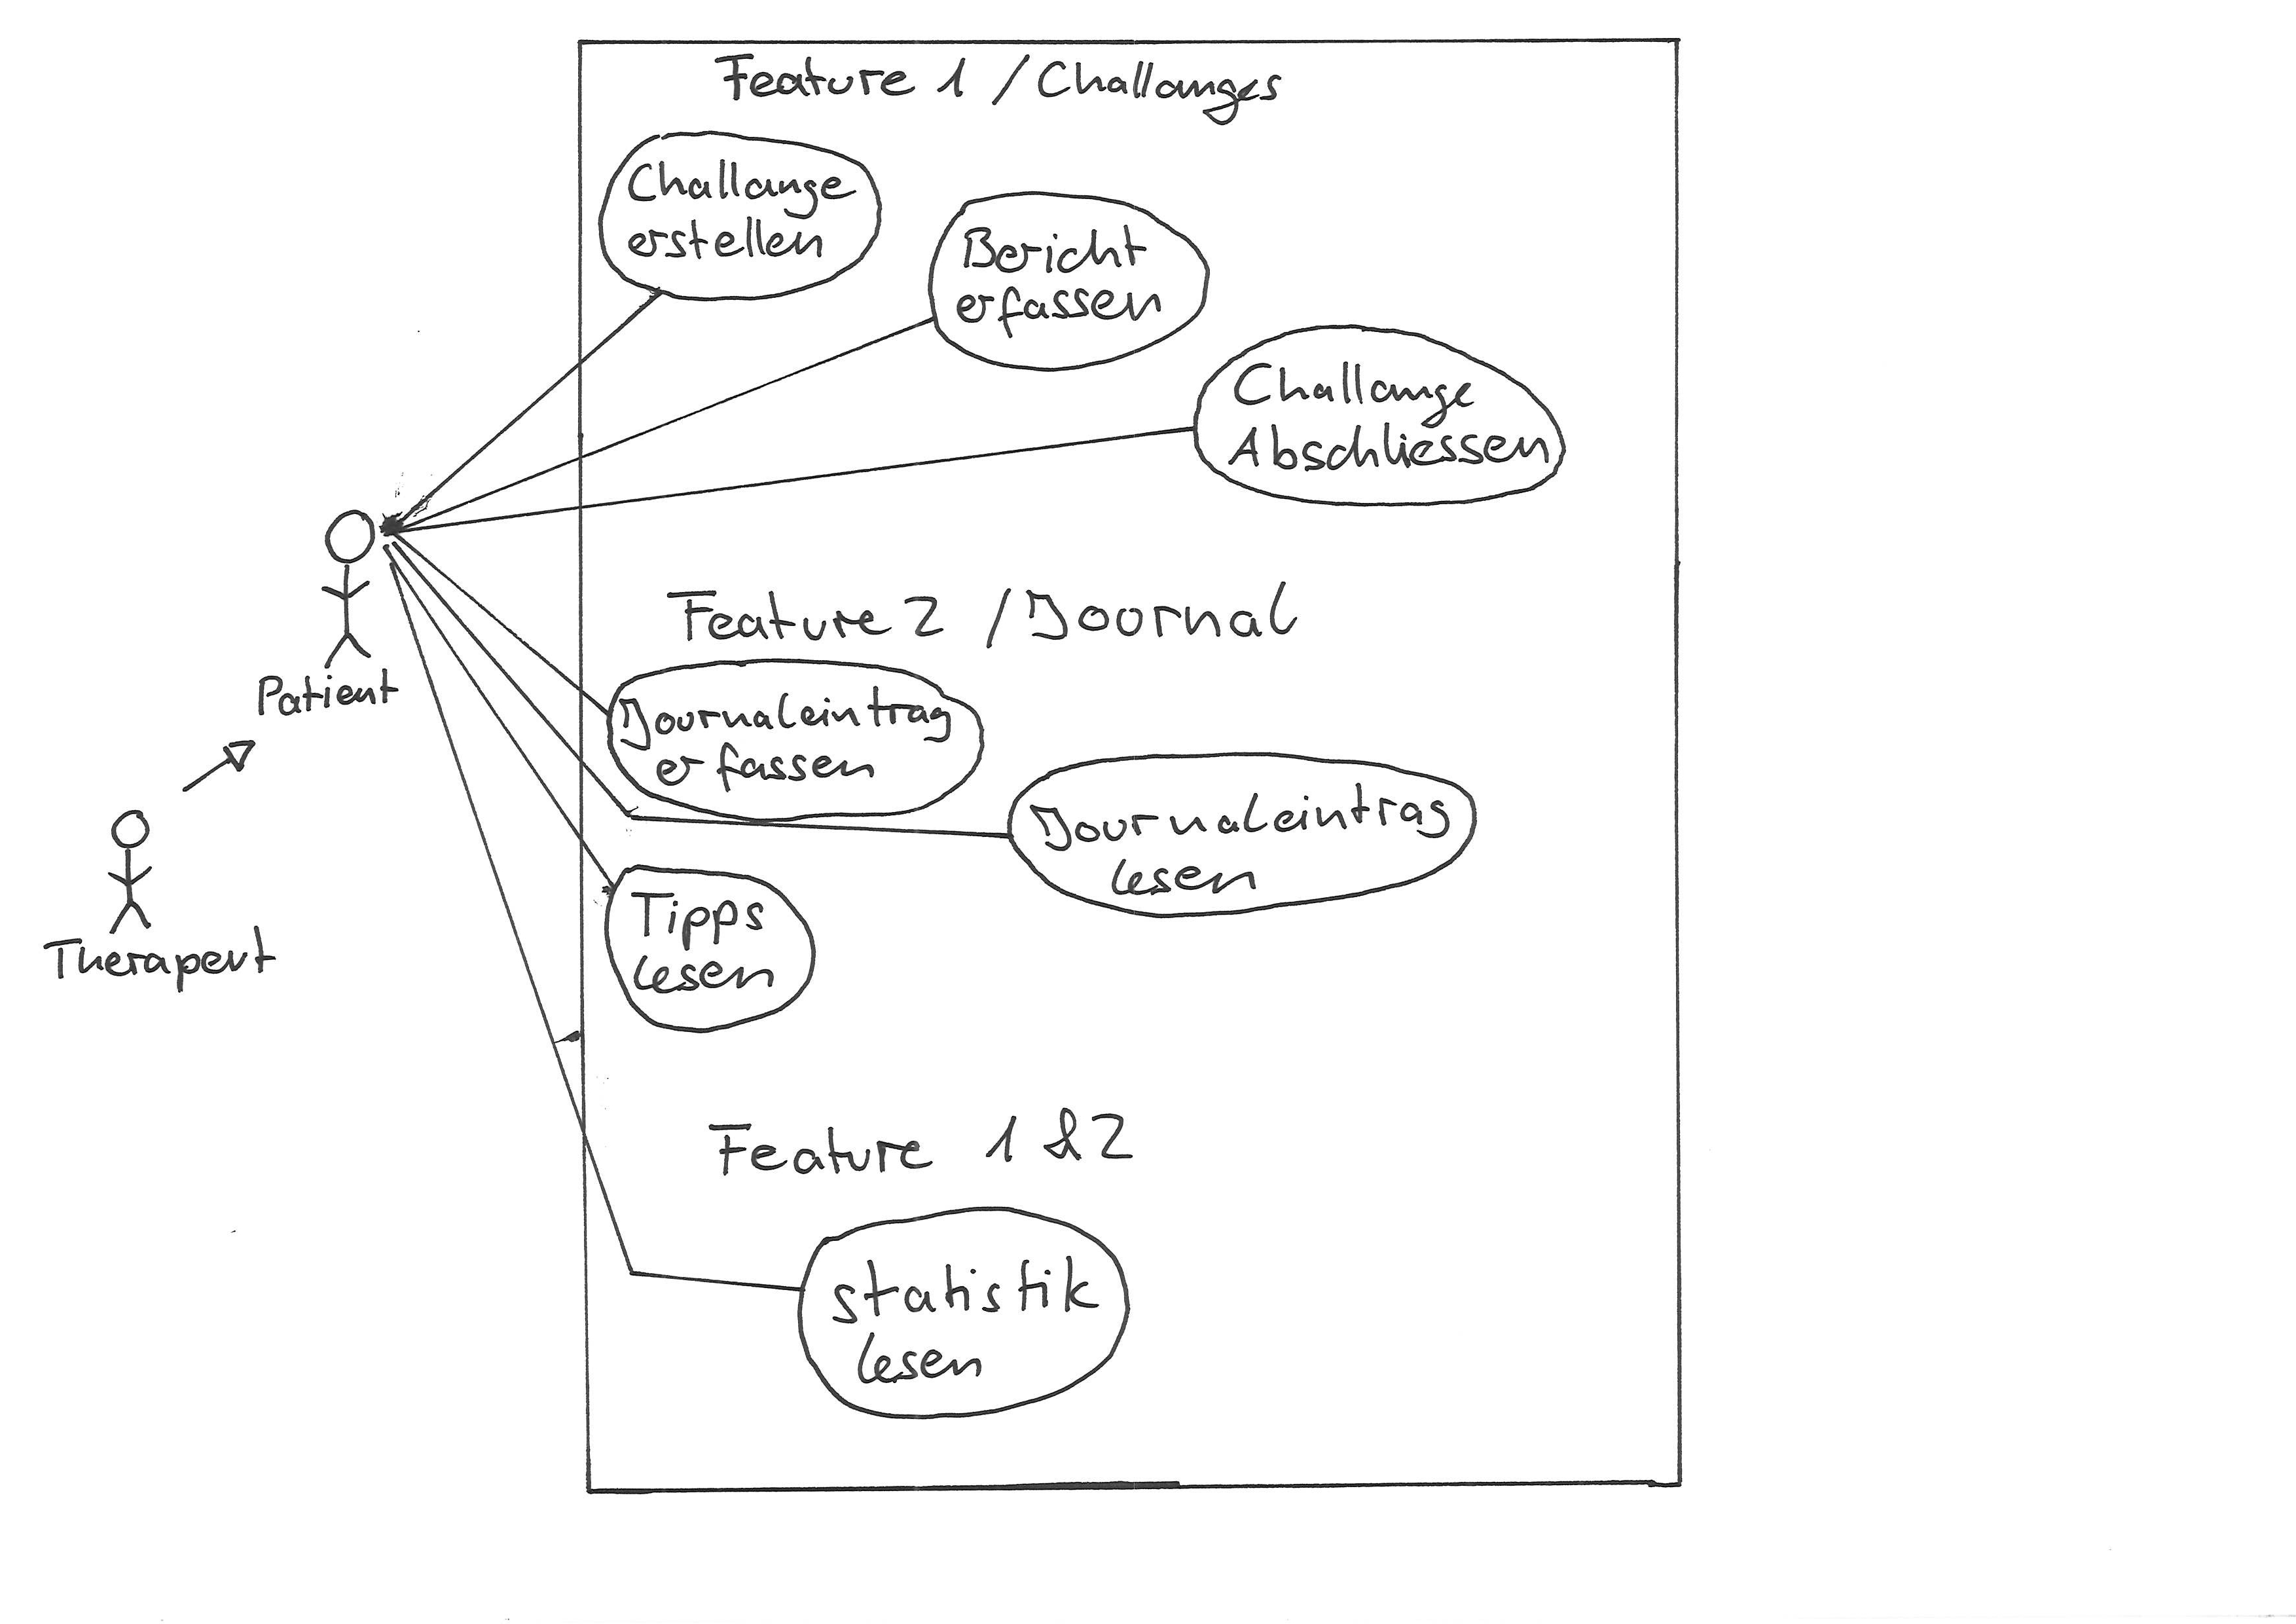
\includegraphics[width=1\textwidth]{UseCaseDiagramm.jpg}
\caption{Use Case Diagramm Feature 1}
\end{figure}

\section{Use Cases}

\subsection{Use Case 1}
\begin{table}[H]
 \caption{Use Case 1}
 \begin{tabularx}{\textwidth}{|l|X|}
     \hline
     \textbf{Bezeichnung}       & \textbf{Beschreibung} \\
     \hline
     Name                       & Challange erstellen \\
     \hline
     Nummer                     & 1 \\
     \hline
     Kurzbeschreibung           & Der Patient erfasst eine neue Challange. \\
     \hline
     Beteiligte Akteure         & Benutzer \\
     \hline
     Ausl\"{o}ser / Vorbedingung    & keine \\
     \hline
     Ergebnisse / Nachbedingung & Die Challange erscheint im richtigen Level mit dem richtigen Status. Sie wird f\"{u}r die Statistik ber\"{u}cksichtigt. \\
     \hline
 \end{tabularx}
 \label{table: Use Case 1}
\end{table}

\section{Ablauf}
\begin{table}[H]
 \caption{Version}
 \begin{tabularx}{\textwidth}{|l|l|X|}
     \hline
     \textbf{Nr.} & \textbf{Akteur} & \textbf{Aktion} \\
     \hline
     1.0          & Benutzer        & Der Patient bet\"{a}tigt den Hinzuf\"{u}gen Buttton. \\
     \hline
     1.1          & Benutzer        & \"{U}ber die Erstellungsmaske werden die Details f\"{u}r die Challange abgef\"{u}llt. Danach wird die Challange gespeichert. \\
     \hline
     1.2          & System          & \"{U}berpr\"{u}fung der eingegebenen Daten.  \\
     \hline
     1.3          & System          & Die Challange wird dem dazugeh\"{o}rigen Level angef\"{u}gt und auf dem UI angezeigt. \\
     \hline
 \end{tabularx}
 \label{table: Version}
\end{table}

\subsection{Use Case 2}
\begin{table}[H]
 \caption{Use Case 2}
 \begin{tabularx}{\textwidth}{|l|X|}
     \hline
     \textbf{Bezeichnung}       & \textbf{Beschreibung} \\
     \hline
     Name                       & Neuer Journaleintrag \\
     \hline
     Nummer                     & 2 \\
     \hline
     Kurzbeschreibung           & Der Patient erfasst einen neuen Journaleintrag. \\
     \hline
     Beteiligte Akteure         & Benutzer \\
     \hline
     Ausl\"{o}ser / Vorbedingung    & keine \\
     \hline
     Ergebnisse / Nachbedingung & Der Journal eintrag wird erstellt und ist in der \"{U}bersicht der Journaleintr\"{a}ge ersichtlich. Der neue Journaleintrag wird f\"{u}r die Statistik ber\"{u}cksichtigt. \\
     \hline
 \end{tabularx}
 \label{table: Use Case 2}
\end{table}

\subsubsection{Ablauf}
\begin{table}[H]
 \caption{Version}
 \begin{tabularx}{\textwidth}{|l|l|X|}
     \hline
     \textbf{Nr.} & \textbf{Akteur} & \textbf{Aktion} \\
     \hline
     1.0          & Benutzer        & Der Benutzer w\"{a}hlt den Hinzuf\"{u}gen Button. \\
     \hline
     1.1          & Benutzer        & \"{U}ber die Erstellungsmaske werden die Details f\"{u}r den Journaleintrag eingef\"{u}gt. Danch wird er gespeichert. \\
     \hline
     1.2          & System          & \"{U}berpr\"{u}fung der eingegebenen Daten.  \\
     \hline
     1.3          & System          & Der Eintrag wird denn bestehenden Eintr\"{a}gen angef\"{u}gt und im UI dargestellt. \\
     \hline
 \end{tabularx}
 \label{table: Version}
\end{table}
